\documentclass[bachelor]{thesis-uestc}
\usepackage{indentfirst}
\usepackage{amssymb, amsmath}
\usepackage{graphicx, subfigure}
\usepackage{algorithm, algorithmic, float}
% 没有使用thesis-uestc的算法模板, 需将thesis-uestc中的相关内容注释掉, 避免冲突
\usepackage{listings}
\usepackage{fancyhdr}
\usepackage{booktabs}

% ----------------------------------------- Document -----------------------------------------

\begin{document}

% ----------------------------------------- 目录 -----------------------------------------
\thesistableofcontents

% ----------------------------------------- 正文 -----------------------------------------
\thesischapterexordium % 需求分析

\section{总体要求}
\begin{itemize}
	\item 存储一张表,然后能对该表进行查询、添加等操作。上述功能以API的形式提供给应用使用。
\end{itemize}

\begin{figure}[htbp]
	\centering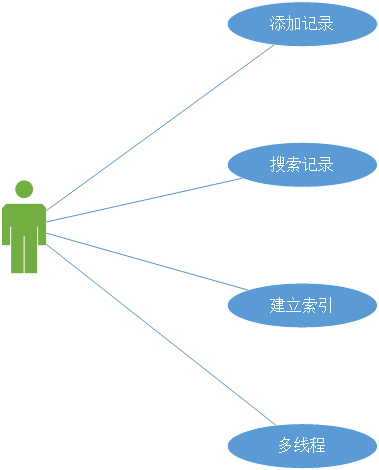
\includegraphics[height=6cm]{images/use_case.png}
	\caption{用例图}
	\label{fig:use_case}
\end{figure}

\section{存储要求}
\begin{itemize}
	\item 存储一张表,然后能对该表进行查询、添加等操作。上述功能以API的形式提供给应用使用。
	\item 该表有100个属性,每个属性都是int64\_t类型;
	\item 需要支持的最大行数为1百万行。
\end{itemize}

\section{添加要求}
\begin{itemize}
	\item 提供API函数,实现向表格添加一行的功能(添加到表格的末尾)。
\end{itemize}

\section{搜索要求}
\begin{itemize}
	\item 提供API函数,实现对表格的某一个属性进行范围查找的功能。例如:查找在属性A上,大于等于50,小于等于100的所有行
	\item 用户可以指定在哪一个属性上进行搜索;
	\item 当搜索结果包含的行数过多时,可以只返回一小部分,如10行等。
\end{itemize}

\section{索引要求}
\begin{itemize}
	\item 提供API函数,为表格的某一个属性建立索引结构,以实现快速搜索;
	\item 自行选择使用哪种数据结构,建立索引结构,比如B+树等;
	\item 建立的索引结构,需要保存到一个文件中(索引文件);下次重启应用程序,并执行搜索任务时,应先检查是否已为相应属性建立了索引结构;
	\item 即,搜索功能实现时,需要查找是否有索引文件存在,若有,则使用该文件加速搜索。	
\end{itemize}

\section{并发要求}
\begin{itemize}
	\item 应用程序可以以多线程的方式,使用我们提供的上述API;
	\item 要保证多线程环境下,表、索引结构、索引文件的一致性。
\end{itemize}

\chapter{总体设计}
\section{整个程序的架构}
存储引擎维护三个文件:table\_file,index\_file,manifest\_file。其中,table\_file负责用户添加数据的持久化;index\_file负责索引结构的持久化;manifest\_file负责存储元数据,以便重启程序后进行恢复。\par
用户在使用该引擎时可以以多线程方式向表中添加数据和查询数据,但建立索引时必须以单线程方式,因为索引结构属于全局结构,即整个表只有一个索引结构。如果以多线程方式建立索引就会存在一个问题:如果线程A建立了索引,那么这个索引结构只是针对线程A所添加的数据而建立的;如果线程B被调度,并且尝试建立索引,那么线程A建立的索引就会需要合并上线程B添加的数据所对应的索引。当多个线程并发地添加数据并尝试建立索引时,索引结构就会被频繁修改,造成效率的降低。基于上述考虑,该存储引擎在设计时只允许以单线程的方式建立索引,如果多线程并发添加数据,那么必须等到所有线程结束后再给表中的属性建立索引。\par
另外,索引结构只有一个,也就是说同一时刻只存在表中的某一个属性的索引。当尝试为别的属性建立索引时,旧的索引结构就会被删除。\par
存储引擎在开发时进行了跨平台处理,支持Linux和Windows平台。

\section{关键流程分析}
\subsection{添加数据}
添加数据的流程图如图\ref{fig:append}所示。因为添加数据要实现多线程安全,所以需要先获得互斥锁,然后判断table\_file文件是否有效、用户输入是否有效等,检查成功后就可以将编码后的数据使用追加写的方式写入table\_file。

\begin{figure}[htbp]
	\centering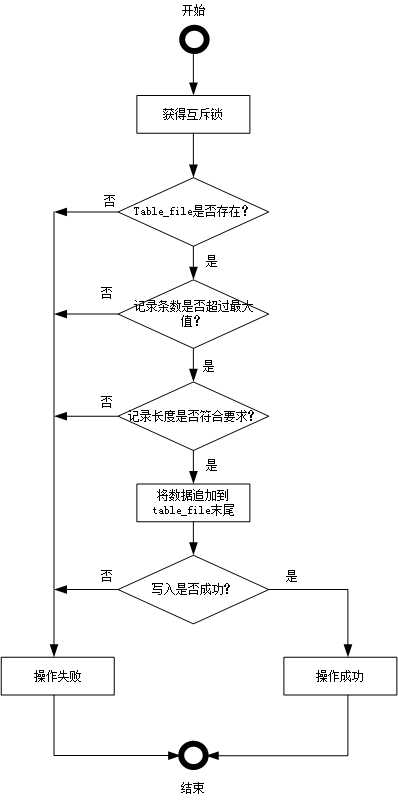
\includegraphics[height=10cm]{images/append.png}
	\caption{添加数据}
	\label{fig:append}
\end{figure}

\subsection{建立索引}
建立索引的流程图如图\ref{fig:build_index}所示。为标号为attr\_id所对应的属性列建立索引时,如果用户没有显式告知存储引擎,添加数据已经结束,那么程序就主动结束数据的添加,关闭可写的table\_file文件,并重新以只读方式打开table\_file。然后从table\_file读入需要建立索引的属性列的全部数据,构造一个IndexEntry结构的线性表(IndexEntry结构包含两个数据,一个是表中的数据,一个是该数据所在的行号),将其排序后写入index\_file。写入成功后重新打开一个只读的index\_file以便后续的查询操作所使用。

\begin{figure}[htbp]
	\centering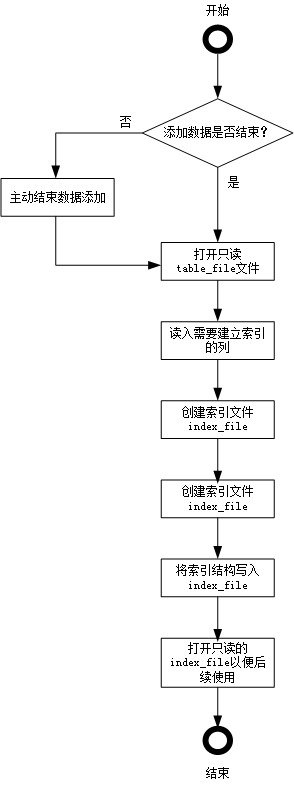
\includegraphics[height=10cm]{images/build_index.png}
	\caption{建立索引}
	\label{fig:build_index}
\end{figure}

\subsection{查询数据}
查询数据时用户需要指定一个属性,以及在该属性上查询的范围。如果索引文件不存在就直接读取表数据文件进行顺序查找,每次读取一行数据(100个属性),判断给定属性的值是否在用户指定的查询区间内,如果是,就说明将该行数据添加到查询结果中。如果索引文件存在,就可以加速查询。因为索引结构实则是一个KV结构的数组,Key就是相应属性上的值,Value就是该属性值所属的行号,根据行号可以实现表数据文件table\_file的随机读取。查询数据的具体流程如图\ref{fig:lookup}所示。

\begin{figure}[htbp]
	\centering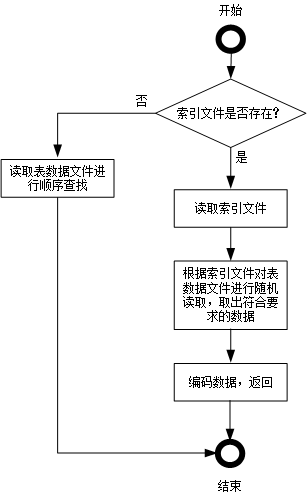
\includegraphics[height=10cm]{images/lookup.png}
	\caption{查询数据}
	\label{fig:lookup}
\end{figure}

\chapter{详细设计与实现}
\section{文件I/O与跨平台}
存储引擎只支持两种类型的文件:写入方式只能是追加写的可写文件WritableFile,支持随机读的只读文件RandomAccessFile。这两个文件抽象类对Linux和Windows都有具体的实现,跨平台的核心就是底层的文件操作接口。相关类图如图\ref{fig:randonaccessfile}和图\ref{fig:writablefile}所示。

\begin{figure}[htbp]
	\centering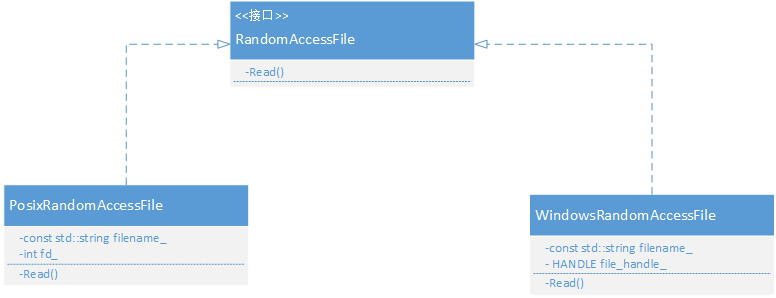
\includegraphics[height=5cm]{images/randomaccessfile.png}
	\caption{RandomAccessFile类图}
	\label{fig:randonaccessfile}
\end{figure}

在PosixRandomAccessFile中,成员变量fd\_是int类型的文件描述符;在WindowsRandomAccessFile中,file\_handle\_是HANDLE类型的文件句柄,二者的实质都是进程的文件指针表的索引(下标)。

\begin{figure}[htbp]
	\centering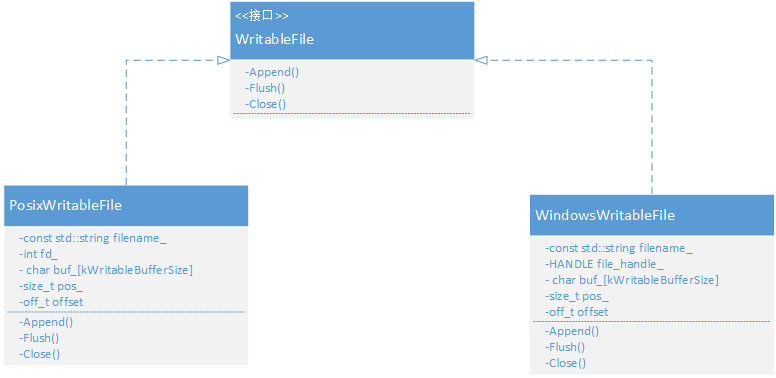
\includegraphics[height=5cm]{images/writablefile.png}
	\caption{WritableFile类图}
	\label{fig:writablefile}
\end{figure}

在WritableFile的两个子类中,buf\_是写缓冲,每次接受到文件写请求时都先将数据写入缓冲区,待缓冲区满后在写入磁盘;pos\_表示当前缓冲区内的数据写到哪里了;offset\_是文件的磁盘偏移,等价于文件的当前大小,每次Flush数据到磁盘时都会更新offset\_。

抽象基类RandomAccessFile/WritableFile的子类实例分别由抽象基类Env的子类WindowsEnv/PosixEnv实例创建,这里使用的是工厂方法模式。Env及其子类的类图如图\ref{fig:env}所示。

\begin{figure}[htbp]
	\centering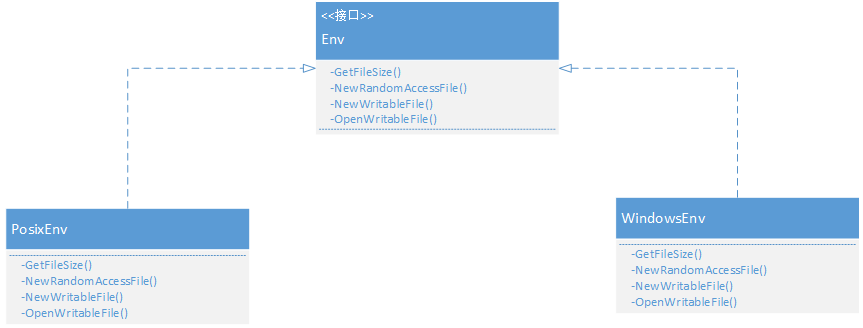
\includegraphics[height=5cm]{images/env.png}
	\caption{Env类图}
	\label{fig:env}
\end{figure}

\subsection{文件I/O设计与实现}
\subsubsection{文件随机读}
Linux平台上,PosixRandomAccessFile::Read()使用pread()系统调用根据给定的偏移量随机读;Windows平台上,WindowsRandomAccessFile::Read()使用ReadFile()和参数OVERLAPPED实现随机读。

\subsubsection{文件追加写}
调用WritableFile::Append()写文件时先将数据写入内存缓冲,当缓冲区满后再Flush到磁盘,以此减少磁盘I/O次数提高效率。

\subsection{Env工厂方法具体实现}
抽象基类Env提供了4个接口:GetFileSize()获取文件大小;NewRandomAccessFile()创建一个RandomAccessFile子类实例;NewWritableFile()和OpenWritableFile()都是创建一个WritableFile子类实例,是不过New*会新建一个文件;Open*打开一个已存在的文件,并将文件指针移到文件末尾。\par
Linux平台上PosixEnv::GetFileSize()使用stat()系统调用,Windows平台上WindowsEnv::GetFileSize()先使用CreateFile()打开文件,获得文件句柄,再使用GetFileSize()系统调用获得文件大小,最后CloseHandle()关闭文件句柄。\par
Linux平台上PosixEnv::NewRandomAccessFile()/NewWritableFile()使用open()系统调用打开文件,Windows平台上WindowsEnv::NewRandomAccessFile()/NewWritableFile()使用CreateFile()系统调用打开文件。这里需要注意,Linux的open()打开的文件默认是非阻塞的,即文件打开到关闭期间,可以调用open()再次打开之;但是Windows需要给CreateFile()指定FILE\_SHARE\_READ或FILE\_SHARE\_WRITE显式地创建为非阻塞模式,否则在关闭文件前无法再次打开之。\par
PosixEnv和WindiwsEnv的代码如下:
\begin{lstlisting}[language=C++, basicstyle=\ttfamily\tiny, numbers=left, numberstyle=\tiny, keywordstyle=\color{blue!70}, commentstyle=\color{red!50!green!50!blue!50}, frame=shadowbox, rulesepcolor=\color{red!20!green!20!blue!20}]
class PosixEnv : public Env {
public:
    PosixEnv() = default;
    PosixEnv(const PosixEnv &) = delete;
    PosixEnv &operator=(const PosixEnv &)= delete;
    ~PosixEnv() = default;

    Status GetFileSize(const std::string &filename, size_t *size) override {
        struct stat buf;
        if (::stat(filename.c_str(), &buf) >= 0) {
            *size = static_cast<size_t>(buf.st_size);
            return Status::OK();
        }
        *size = 0;
        return Status::IOError();
    }

    Status NewRandomAccessFile(const std::string &filename, RandomAccessFile **result) override {
        int fd = ::open(filename.c_str(), O_RDONLY);
        if (fd < 0) {
            *result = nullptr;
            return Status::IOError();
        }

        *result = new PosixRandomAccessFile(filename, fd);
        return Status::OK();
    }

    Status NewWritableFile(const std::string &filename, WritableFile **result) override {
        int fd = ::open(filename.c_str(), O_RDWR | O_CREAT | O_TRUNC, 0664);
        if (fd < 0) {
            *result = nullptr;
            return Status::IOError();
        }

        *result = new PosixWritableFile(filename, fd);
        return Status::OK();
    }

    Status OpenWritableFile(const std::string &filename, WritableFile **result) override {
        int fd = ::open(filename.c_str(), O_RDWR | O_CREAT | O_APPEND, 0664);
        if (fd < 0) {
            *result = nullptr;
            return Status::IOError();
        }

        *result = new PosixWritableFile(filename, fd);
        return Status::OK();
    }
};

class WindowsEnv : public Env {
public:
    WindowsEnv() = default;
    WindowsEnv(const WindowsEnv &) = delete;
    WindowsEnv &operator=(const WindowsEnv &)= delete;
    ~WindowsEnv() = default;

    Status GetFileSize(const std::string &filename, size_t *size) override {
		HANDLE file_handle = ::CreateFileA(filename.c_str(),
			GENERIC_READ,
			FILE_SHARE_READ | FILE_SHARE_WRITE,
			nullptr,
			OPEN_EXISTING,
			FILE_ATTRIBUTE_NORMAL,
			0);
		if (file_handle == INVALID_HANDLE_VALUE) {
		    *size = 0;
			return Status::IOError();
		}
		*size = ::GetFileSize(file_handle, nullptr);
		::CloseHandle(file_handle);
        return Status::OK();
    }

    Status NewRandomAccessFile(const std::string &filename, RandomAccessFile **result) override {
		HANDLE file_handle = ::CreateFileA(filename.c_str(),
			GENERIC_READ, 
			FILE_SHARE_READ | FILE_SHARE_WRITE, 
			nullptr,
			OPEN_EXISTING, 
			FILE_ATTRIBUTE_NORMAL, 
			0);
		if (file_handle == INVALID_HANDLE_VALUE) {
		    *result = nullptr;
			return Status::IOError();
		}

        *result = new WindowsRandomAccessFile(filename, file_handle);
        return Status::OK();
    }

	Status NewWritableFile(const std::string &filename, WritableFile **result) override {
		HANDLE file_handle = ::CreateFileA(filename.c_str(),
			GENERIC_READ | GENERIC_WRITE,
			FILE_SHARE_READ | FILE_SHARE_WRITE,
			nullptr,
			CREATE_ALWAYS,
			FILE_ATTRIBUTE_NORMAL | FILE_FLAG_WRITE_THROUGH,
			0);
		if (file_handle == INVALID_HANDLE_VALUE) {
		    *result = nullptr;
			return Status::IOError();
		}

		*result = new WindowsWritableFile(filename, file_handle);
		return Status::OK();
	}

	Status OpenWritableFile(const std::string &filename, WritableFile **result) override {
		HANDLE file_handle = ::CreateFileA(filename.c_str(),
			GENERIC_READ | GENERIC_WRITE,
			FILE_SHARE_READ | FILE_SHARE_WRITE,
			nullptr,
			OPEN_ALWAYS,
			FILE_ATTRIBUTE_NORMAL | FILE_FLAG_WRITE_THROUGH,
			0);
		if (file_handle == INVALID_HANDLE_VALUE) {
		    *result = nullptr;
			return Status::IOError();
		}
		if (GetLastError() == ERROR_ALREADY_EXISTS) {
			if (INVALID_SET_FILE_POINTER == ::SetFilePointer(file_handle, 0, nullptr, FILE_END)) {
		        *result = nullptr;
				return Status::IOError();
			}
		}

        *result = new WindowsWritableFile(filename, file_handle);
        return Status::OK();
    }
};
\end{lstlisting}

\section{表数据操作设计与实现}
表数据的具体操作包括添加数据、建立索引和范围查询,以上操作需要实现多线程安全。Table类对此进行了封装,类图如图\ref{fig:table}所示。

\begin{figure}[htbp]
	\centering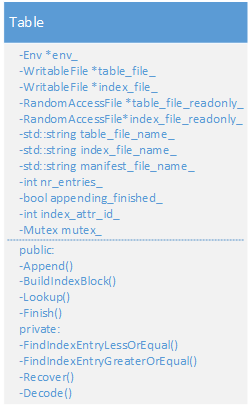
\includegraphics[height=7cm]{images/table.png}
	\caption{Table类图}
	\label{fig:table}
\end{figure}

\begin{itemize}
	\item 成员变量:
	\begin{itemize}
		\item Env *env\_ 工厂类,根据不同的平台创建不同子类类型的RandomAccessFile/WritableFile子类实例;
		\item WritableFile *table\_file\_, *index\_file\_ 可写的表数据文件和索引文件,在向表中添加数据和建立索引结构时使用之;
		\item RandomAccessFile **table\_file\_readonly\_, *index\_file\_readonly\_ 只读的表数据文件和索引文件,在查询数据时使用之;
		\item std::string table\_file\_name\_, index\_file\_name\_, manifest\_file\_name 表数据文件、索引文件和存储元信息的MANIFEST文件名;
		\item int nr\_entries\_ 表数据文件中存储了多少条数据;
		\item bool appending\_finished 向表中添加数据的操作是否已经结束;
		\item int index\_attr\_id\_ 当前索引结构/索引文件是为哪个属性列建立的;
		\item Mutex mutex\_ 互斥量,向表中添加数据时需要先获得互斥锁。Mutex类只是对std::mutex的轻量级封装,需要配合MutexLock类进行使用。
	\end{itemize}
	\item 成员函数:
	\begin{itemize}
		\item Status Append(std::vector<uint64\_t> \&data) 向表中添加数据,data的长度要求等于Table::kNumTableAttributes(100);
		\item Status BuildIndexBlock(int attr\_id) 为属性列attr\_id建立索引结构,并将其保存到文件中;
		\item Status Lookup(int attr\_id, uint64\_t lower\_bound, uint64\_t upper\_bound, std:: vector<std::vector<uint64\_t>> *results) 在属性列attr\_id上查找[lower\_bound, upper\_bound]范围内的数据,将符合要求的行返回到results;
		\item Status Finish() 结束向表中添加数据,并创建MANIFEST文件,向其中写入nr\_entries\_和index\_attr\_id\_;
		\item int FindIndexEntryLessOrEqual(std::vector<IndexEntry> \&index\_entries, uint64\_t x) const 使用二分查找方式在index\_entries中查找Key刚好小于或等于x的IndexEntry;
		\item int FindIndexEntryGreaterOrEqual(std::vector<IndexEntry> \&index\_entries, uint64\_t x) const 使用二分查找方式在index\_entries中查找Key刚好大于或等于x的IndexEntry;
		\item Status Recover() 每次重启程序时:如果表数据文件存在就打开之,用于后续的写入;读取MENIFEST文件,恢复nr\_entries\_和index\_attr\_id\_;
		\item std::vector<uint64\_t> Decode(const Slice \&slice) const 将Slice对象指向的字符数组解码成uint64\_t数组。
	\end{itemize}
\end{itemize}

\subsection{添加数据}
Table::Append()负责将数据添加到表的末尾。如果表数据文件无效,或者记录的条数已达最大值,或者用户输入的数据长度不合法,就直接返回相应的错误信息。如果没有任何异常,就可以进行数据的添加操作。首先需要获得互斥锁,然后调用PutFixed64()将用户输入的100个uint64\_t数据编码成字符数组的形式(字符数组使用std::string来实现),再调用WritableFile实例table\_file\_的Append()方法完成文件写入,最后计数器nr\_entries\_递增。相应代码如下:

\begin{lstlisting}[language=C++, basicstyle=\ttfamily\tiny, numbers=left, numberstyle=\tiny, keywordstyle=\color{blue!70}, commentstyle=\color{red!50!green!50!blue!50}, frame=shadowbox, rulesepcolor=\color{red!20!green!20!blue!20}]
Status Table::Append(std::vector<uint64_t> &data) {
	MutexLock l(&mutex_);
	if (table_file_ == nullptr) {
		return Status::GeneralError("Table::table_file_ has been closed.");
	}
	if (nr_entries_ >= kMaxTableEntries) {
		return Status::GeneralError("too much data");
	}
	assert(data.size() == kNumTableAttributes);
	std::string d;
	for (int i = 0; i < kNumTableAttributes; i++) {
		PutFixed64(&d, data[i]);
	}
	
	Status status = table_file_->Append(d);
	if (!status.ok()) {
		return status;
	}
	nr_entries_++;
	return Status::OK();
}
\end{lstlisting}

\subsection{建立索引}
\begin{figure}[htbp]
	\centering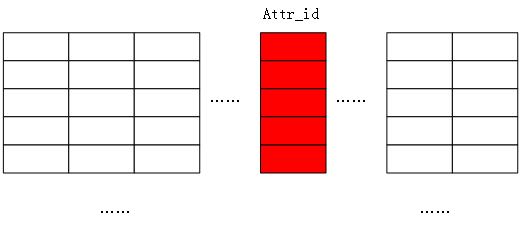
\includegraphics[height=4cm]{images/index_demo.png}
	\caption{Demo:为Attr\_id属性列建立索引}
	\label{fig:index_demo}
\end{figure}

Table::BuildIndexBlock()负责建立索引结构并将其保存到文件。首先读入表数据文件的某一属性列attr\_id(如图\ref{fig:index_demo}所示),将其作为Key,并将所属行号作为Value,封装成一个IndexEntry的KV结构index\_entries。然后将根据Key排序后的index\_entries编码成字符数组的形式写入索引文件index\_file。相应代码如下:

\begin{lstlisting}[language=C++, basicstyle=\ttfamily\tiny, numbers=left, numberstyle=\tiny, keywordstyle=\color{blue!70}, commentstyle=\color{red!50!green!50!blue!50}, frame=shadowbox, rulesepcolor=\color{red!20!green!20!blue!20}]
Status Table::BuildIndexBlock(int attr_id) {
	Status status;
	if (!appending_finished_) { /* 添加数据结束后才建立索引 */
		Finish();
	}
	assert(attr_id >= 0 && attr_id < kNumTableAttributes);
	index_attr_id_ = attr_id;
	
	if (table_file_readonly_ == nullptr) {
		status = env_->NewRandomAccessFile(table_file_name_, &table_file_readonly_);
		if (!status.ok()) {
			return status;
		}
	}
	
	/* 将attr_id所对应的列读入index_entries */
	Slice result;
	char scratch[sizeof(uint64_t)];
	uint64_t offset = attr_id * sizeof(uint64_t);
	std::vector<IndexEntry> index_entries;
	for (int i = 0; i < nr_entries_; i++) {
		status = table_file_readonly_->Read(offset, sizeof(uint64_t), scratch, &result);
		if (!status.ok()) {
			return status;
		}
		index_entries.push_back(std::make_pair(
			DecodeFixed64(result.data()), i));
		offset += kNumTableAttributes * sizeof(uint64_t);
	}
	
	if (index_file_ == nullptr) {
		status = env_->NewWritableFile(index_file_name_, &index_file_);
		if (!status.ok()) {
			return status;
		}
	}
	
	/* index_entries排序后写入索引文件index_file_ */
	std::sort(index_entries.begin(), index_entries.end());
	std::string d;
	for (size_t i = 0; i < index_entries.size(); i++) {
		PutFixed64(&d, index_entries[i].first);
		PutFixed32(&d, index_entries[i].second);
	}
	
	status = index_file_->Append(d);
	if (status.ok()) {
		status = index_file_->Close();
		if (status.ok()) {
			/* 打开只读的index_file_以便后续使用 */
			if (index_file_readonly_ == nullptr) {
				status = env_->NewRandomAccessFile(index_file_name_, &index_file_readonly_);
			}
		}
	}
	return status;
}
\end{lstlisting}

\subsection{查询数据}
 Table::Lookup()查询数据时首先检查相应属性对因的索引文件是否存在,如果不存在就直接读取表数据文件进行逐行查找,效率较低。如果索引文件存在,就可以在索引结构上进行二分查找,确定符合要求的数据的行号,然后就可以对表数据文件进行随机读,将读入的数据编码后返回给用户。相应代码如下:
 
 \begin{lstlisting}[language=C++, basicstyle=\ttfamily\tiny, numbers=left, numberstyle=\tiny, keywordstyle=\color{blue!70}, commentstyle=\color{red!50!green!50!blue!50}, frame=shadowbox, rulesepcolor=\color{red!20!green!20!blue!20}]
 Status Table::Lookup(int attr_id, uint64_t lower_bound, uint64_t upper_bound,
 	std::vector<std::vector<uint64_t>> *results) {
	 Status status;
	 Slice slice;
	 char scratch[kNumTableAttributes * sizeof(uint64_t)];
 
	 if (table_file_ != nullptr) {
	 assert(!appending_finished_);
	 	table_file_->Flush();
	 }
 
 	if (index_attr_id_ != attr_id ||
 		index_file_readonly_ == nullptr) { /* 索引不存在则读取table_file进行顺序查找 */
 		if (table_file_readonly_ == nullptr) {
 			status = env_->NewRandomAccessFile(table_file_name_, &table_file_readonly_);
 			if (!status.ok()) {
 				return status;
 			}
 		}
 		uint64_t offset = 0;
 		for (int i = 0; i < nr_entries_; i++) {
			status = table_file_readonly_->Read(offset, sizeof(scratch), scratch, &slice);
 			if (!status.ok()) {
 				return status;
 			}
 			std::vector<uint64_t> r = Decode(slice);
			if (r[attr_id] >= lower_bound && r[attr_id] <= upper_bound) {
			 	results->push_back(r);
			}
 			offset += kNumTableAttributes * sizeof(uint64_t);
 		}
 		return status;
 	}
 
	 assert(table_file_readonly_ != nullptr);
	 assert(index_file_readonly_ != nullptr);
	 
	 std::vector<IndexEntry> index_entries;
	 uint64_t offset = 0;
	 for (int i = 0; i < nr_entries_; i++) {
	 	status = index_file_readonly_->Read(offset, sizeof(uint64_t), scratch, &slice);
	 	if (!status.ok()) {
	 		return status;
		}
 		uint64_t var = DecodeFixed64(slice.data());
 		status = index_file_readonly_->Read(offset + sizeof(uint64_t), sizeof(uint32_t), scratch, &slice);
 		if (!status.ok()) {
 			return status;
 		}
 		uint32_t index = DecodeFixed32(slice.data());
 		index_entries.push_back(std::make_pair(var, index));
 		offset += sizeof(uint64_t) + sizeof(uint32_t);
 	}
 
	 int lower_bound_idx = FindIndexEntryGreaterOrEqual(index_entries, lower_bound);
	 int upper_bound_idx = FindIndexEntryLessOrEqual(index_entries, upper_bound);
	 if (lower_bound_idx == -1 || upper_bound_idx == -1) {
	 	return Status::NotFound();
	 }
 
	 for (int i = lower_bound_idx; i <= upper_bound_idx; i++) {
		 const size_t nbytes_per_record = kNumTableAttributes * sizeof(uint64_t);
		 status = table_file_readonly_->Read(index_entries[i].second * nbytes_per_record,
	 	 nbytes_per_record, scratch, &slice);
		 if (!status.ok()) {
		 	return status;
		 }
		 std::vector<uint64_t> r = Decode(slice);
		 results->push_back(r);
	 }
	 return status;
 }
 \end{lstlisting}

\subsection{多线程安全}
多线程安全主要由两个类实现:Mutex和MutexLock,类图如图\ref{fig:mutexlock}所示。

\begin{figure}[htbp]
	\centering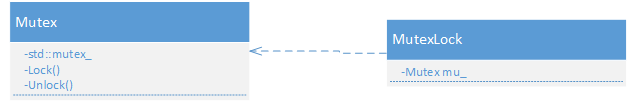
\includegraphics[height=2cm]{images/mutexlock.png}
	\caption{MutexLock类图}
	\label{fig:mutexlock}
\end{figure}

Mutex只是对std::mutex的轻量级封装,需要配合MutexLock使用。 创建MutexLock对象是,构造函数即完成Mutex的Lock()操作;MutexLock对象析构时完成Mutex的Unlock()操作。Mutex/MutexLock的设计参考了LevelDB,相应代码如下:

\begin{lstlisting}[language=C++, basicstyle=\ttfamily\tiny, numbers=left, numberstyle=\tiny, keywordstyle=\color{blue!70}, commentstyle=\color{red!50!green!50!blue!50}, frame=shadowbox, rulesepcolor=\color{red!20!green!20!blue!20}]
class Mutex {
public:
	Mutex() = default;
	~Mutex() = default;
	
	Mutex(const Mutex&) = delete;
	Mutex &operator=(const Mutex&) = delete;
	
	void Lock() { mu_.lock(); }
	void Unlock() { mu_.unlock(); }
private:
	std::mutex mu_;
};

class MutexLock {
public:
	MutexLock(Mutex *mu):mu_(mu) { mu_->Lock(); }
	~MutexLock() { mu_->Unlock(); }
	
	MutexLock(const MutexLock&) = delete;
	MutexLock &operator=(const MutexLock&) = delete;
private:
	Mutex *mu_;
};
\end{lstlisting}

\section{其他}
\subsection{Slice类}
LevelDB中的数据都是用Slice类封装,因为只是保存了指针,不存在数据的深拷贝,所以在传递参数时开销非常小。类图如图\ref{fig:slice}所示。

\begin{figure}[htbp]
	\centering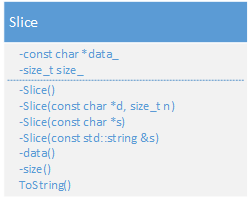
\includegraphics[height=5cm]{images/slice.png}
	\caption{Slice类图}
	\label{fig:slice}
\end{figure}

Slice类提供了4个构造函数,用户可以创建一个不含任何数据的Slice对象,或者使用给定长度的字符数组、字符串或std::string对象创建Slice对象。指针data\_指向具体的数据。

\subsection{Status类}
程序中几乎所有函数的返回值都是Status对象,表示操作是否成功,以及错误类型。类图如图\ref{fig:status}所示。

\begin{figure}[htbp]
	\centering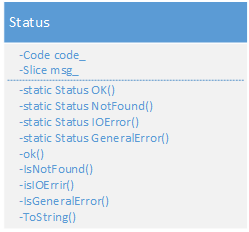
\includegraphics[height=5cm]{images/status.png}
	\caption{Status类图}
	\label{fig:status}
\end{figure}

Status定义了四种操作状态:成功、未找到(主要用于Table的数据查询操作)、I/O错误(文件操作失败)和常规错误(对于常规错误,需要用户自行制定错误消息)。Status类提供了4个static方法用于创建上述4中操作状态对应的Status对象,并提供了对应的非static方法用于判断当前Status对象的状态。同样地,Status类的设计也参考了LevelDB。

\subsection{数据的编码与解码}
在进行数据的存取——写入到文件中、从文件中读取——时,需要进行必要的编码与解码。因此,我参考LevelDB设计以一组32位和64位整数和字符数组之间的编解码函数,如下所示:

\begin{itemize}
	\item void EncodeFixed64(char *dst, uint64\_t value) 将64位无符号整数编码成字符数组,保存到dst指向的内存
	\item void EncodeFixed32(char *dst, uint32\_t value) 将32位无符号整数编码成字符数组,保存到dst指向的内存
	\item void PutFixed64(std::string *dst, uint64\_t value) 将64位无符号整数编码成字符数组,附加到dst的末尾(通过dst->append()实现,下同)
	\item void PutFixed32(std::string *dst, uint32\_t value) 将32位无符号整数编码成字符数组,附加到dst的末尾
	\item uint64\_t DecodeFixed64(const char *ptr) 从ptr解码出一个uint64\_t类型的数据
	\item uint32\_t DecodeFixed32(const char *ptr) 从ptr解码出一个uint32\_t类型的数据
\end{itemize}

\chapter{测试}
\section{测试环境}
\begin{itemize}
	\item 操作系统:Ubuntu 16.04 64位
	\item 硬件:内存4GB
	\item 测试框架:GooglgTest
\end{itemize}

\section{测试内容}
\subsection{测试用例1:单线程}
每次添加1000条记录,每条记录中的100个属性值随机生成;在第1个属性上查询,查询范围是[1000,100000000]。每添加一个数据就执行一次查询,此时的查询操作需要直接读取表数据文件进行,因为索引文件尚未建立。等到所有数据添加结束后,建立索引结构,创建索引文件再次查询,并将查询结果打印出来(最多打印10条记录)。测试中,校验查询结果的方法是:每次添加数据前,先判断相应属性值是否在查询范围内,如果是,就将计数器nr\_expected\_query\_results加一。然后检查Table::Lookup()返回的查询结果的条数是否等于nr\_expected\_query\_results,如果不相等则说明查询结果错误,测试失败;如果相等则还需对所有查询结果逐一检查:每条记录在所给的查询属性上的数值是否落在查询范围内,如果有一条记录不满足则测试失败。\par
另外,测试需要多次进行,目的是测试程序是否能在重启后恢复之前的状态,继续接受添加/查询/建立索引的操作。测试代码如下:

\begin{lstlisting}[language=C++, basicstyle=\ttfamily\tiny, numbers=left, numberstyle=\tiny, keywordstyle=\color{blue!70}, commentstyle=\color{red!50!green!50!blue!50}, frame=shadowbox, rulesepcolor=\color{red!20!green!20!blue!20}]
TEST(table_storage, single_thread1) {
	Table table("table1", "index1", "MANIFEST1");
	TestHelper testhlp;
	Random rnd;
	Status status;
	const int n = 1000;
	const uint64_t lower_bound = 1000;
	const uint64_t upper_bound = 100000000;
	int query_attr_id = 0;
	size_t nr_expected_query_results = 0;
	std::vector<std::vector<uint64_t>> query_results;
	clock_t start, end;
	
	/* 从data文件读取上次的查询结果数, 如果data文件存在的话 */
	testhlp.LoadLastQueryResultsFromFile("data1", reinterpret_cast<int*>(&nr_expected_query_results));
	
	/* 向表中添加数据 */
	start = clock();
	std::cout << "Appending data...\n";
	for (int i = 0; i < n; i++) {
		/* 添加记录 */
		std::vector<uint64_t> nums = rnd.GenerateRandomNumbers(Table::kNumTableAttributes);
		status = table.Append(nums);
		ASSERT_TRUE(status.ok());
	
		/* 添加的记录是否应该在后续的查询结果中出现? */
		if (nums[query_attr_id] >= lower_bound && nums[query_attr_id] <= upper_bound) {
			nr_expected_query_results++;
		}
	
		/* 在query_attr_id指定的属性上进行范围查找. 由于索引未建立, 查询时需要读取table_file */
		query_results.clear();
		status = table.Lookup(query_attr_id, lower_bound, upper_bound, &query_results);
		if (!status.ok()) {
			ASSERT_TRUE(status.IsNotFound());
		}
	}
	
	/* 校验查询结果 */
	ASSERT_EQ(query_results.size(), nr_expected_query_results);
	for (size_t i = 0; i < query_results.size(); i++) {
		ASSERT_EQ(query_results[i].size(), Table::kNumTableAttributes);
		ASSERT_TRUE(query_results[i][query_attr_id] >= lower_bound &&
			query_results[i][query_attr_id] <= upper_bound);
	}
	end = clock();
	printf("Done. Time elapsed: %.5fs\n", (double) (end - start) / CLOCKS_PER_SEC);
	
	/* 将新的查询结果数写入data文件 */
	status = testhlp.SaveLastQueryResultsToFile("data1", static_cast<int>(nr_expected_query_results));
	ASSERT_TRUE(status.ok());
	
	/* 建立索引 */
	status = table.Finish();
	ASSERT_TRUE(status.ok());
	status = table.BuildIndexBlock(query_attr_id);
	ASSERT_TRUE(status.ok());
	
	/* 在query_attr_id指定的属性上进行范围查找. 索引已建立, 查询时使用索引加速查找 */
	query_results.clear();
	status = table.Lookup(query_attr_id, lower_bound, upper_bound, &query_results);
	if (!status.ok()) {
		ASSERT_TRUE(status.IsNotFound());
	}
	
	/* 校验查询结果 */
	ASSERT_EQ(query_results.size(), nr_expected_query_results);
	for (size_t i = 0; i < query_results.size(); i++) {
		ASSERT_EQ(query_results[i].size(), Table::kNumTableAttributes);
		ASSERT_TRUE(query_results[i][query_attr_id] >= lower_bound &&
		query_results[i][query_attr_id] <= upper_bound);
	}
	
	/* 打印查询结果. 最多打印10条记录 */
	...
}
\end{lstlisting}

\subsection{测试用例2:多线程}
创建8个线程并发地向表中添加数据,每个线程添加1000/8=125条记录,待线程结束后执行查询(属性列和查询范围和单线程的测试相同)。校验查询结果的过程和测试用例1一致,这里不再赘述。\par
和单线程测试一样,测试需要多次进行,目的是测试程序是否能在重启后恢复之前的状态,继续接受添加/查询/建立索引的操作。测试代码如下:

\begin{lstlisting}[language=C++, basicstyle=\ttfamily\tiny, numbers=left, numberstyle=\tiny, keywordstyle=\color{blue!70}, commentstyle=\color{red!50!green!50!blue!50}, frame=shadowbox, rulesepcolor=\color{red!20!green!20!blue!20}]
TEST(table_storage, multi_thread) {
	TestHelper testhlp;
	Status status;
	const int nr_thds = 8;
	const int n = 1000 / nr_thds;

	/* 从data文件读取上次的查询结果数, 如果data文件存在的话 */
	testhlp.LoadLastQueryResultsFromFile("data0", reinterpret_cast<int*>(&g_nr_expected_query_results));

	/* 创建多个线程 */
	std::thread **thds = new std::thread*[nr_thds];
	for (int i = 0; i < nr_thds; i++) {
		thds[i] = new std::thread(thd_routine, n);
	}
	for (int i = 0; i < nr_thds; i++) {
		thds[i]->join();
	}
	for (int i = 0; i < nr_thds; i++) {
		delete thds[i];
	}
	delete[] thds;

	/* 将新的查询结果数写入data文件 */
	status = testhlp.SaveLastQueryResultsToFile("data0", static_cast<int>(g_nr_expected_query_results));
	ASSERT_TRUE(status.ok());

	/* 在query_attr_id指定的属性上进行范围查找. 由于索引未建立, 查询时需要读取table_file */
	std::vector<std::vector<uint64_t>> query_results;
	status = g_table.Lookup(g_query_attr_id, g_lower_bound, g_upper_bound, &query_results);
	if (!status.ok()) {
		ASSERT_TRUE(status.IsNotFound());
	}

	/* 校验查询结果 */
	ASSERT_EQ(query_results.size(), g_nr_expected_query_results);
	for (size_t i = 0; i < query_results.size(); i++) {
		ASSERT_EQ(query_results[i].size(), Table::kNumTableAttributes);
		ASSERT_TRUE(query_results[i][g_query_attr_id] >= g_lower_bound &&
		query_results[i][g_query_attr_id] <= g_upper_bound);
	}

	/* 建立索引后在次测试查询 */
	g_table.BuildIndexBlock(g_query_attr_id);
	query_results.clear();

	status = g_table.Lookup(g_query_attr_id, g_lower_bound, g_upper_bound, &query_results);
		if (!status.ok()) {
		ASSERT_TRUE(status.IsNotFound());
	}

	/* 校验查询结果 */
	ASSERT_EQ(query_results.size(), g_nr_expected_query_results);
	for (size_t i = 0; i < query_results.size(); i++) {
		ASSERT_EQ(query_results[i].size(), Table::kNumTableAttributes);
		ASSERT_TRUE(query_results[i][g_query_attr_id] >= g_lower_bound &&
		query_results[i][g_query_attr_id] <= g_upper_bound);
	}

	/* 打印查询结果 */
	...
}
\end{lstlisting}

其中,每个线程负责向表中添加数据,代码如下:

\begin{lstlisting}[language=C++, basicstyle=\ttfamily\tiny, numbers=left, numberstyle=\tiny, keywordstyle=\color{blue!70}, commentstyle=\color{red!50!green!50!blue!50}, frame=shadowbox, rulesepcolor=\color{red!20!green!20!blue!20}]
void thd_routine(const int n) {
	Random rnd;
	for (int i = 0; i < n; i++) {
		/* 添加记录 */
		std::vector<uint64_t> nums =
		rnd.GenerateRandomNumbers(Table::kNumTableAttributes);
		Status status = g_table.Append(nums);
		ASSERT_TRUE(status.ok());
		
		/* 添加的记录是否应该在后续的查询结果中出现? */
		if (nums[g_query_attr_id] >= g_lower_bound &&
			nums[g_query_attr_id] <= g_upper_bound) {
			g_nr_expected_query_results++;
		}
	}
}
\end{lstlisting}

g\_nr\_expected\_query\_results是期望的查询结果条数,用于后续校验查询结果。因为该变量被多个线程并发地读写,所以将其声明为原子类型变量std::atomic<size\_t>,以此保证线程安全性。

\section{测试结果}
上述两个测试用例的测试结果如图\ref{fig:test_linux}所示。打印查询结果时最多打印10条,并且只打印所查询的属性列上的数值,其余属性值省略。
\begin{figure}[htbp]
	\centering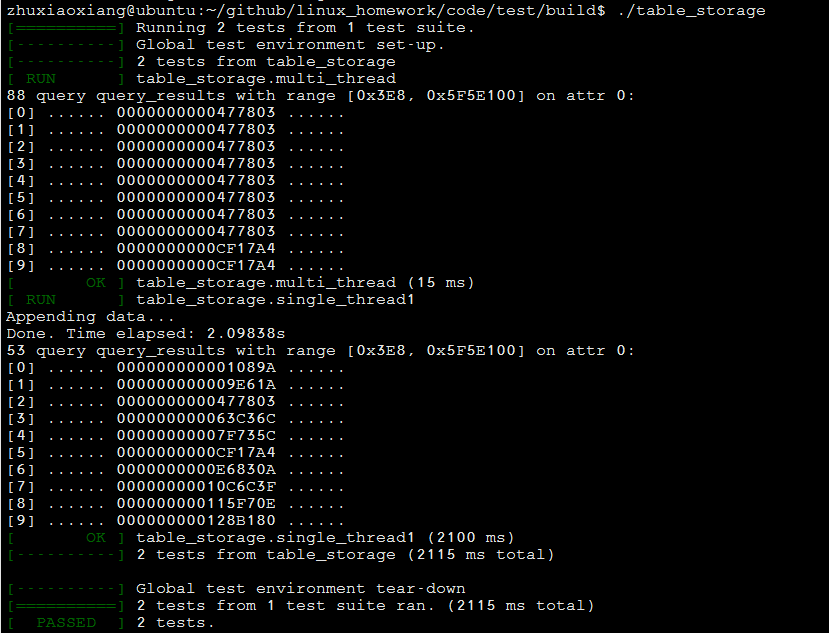
\includegraphics[height=10cm]{images/test_linux.png}
	\caption{测试结果(1)}
	\label{fig:test_linux}
\end{figure}

如图\ref{fig:test_linux}所示,单线程和多线程两个测试用例均测试通过。创建的表数据文件、索引文件以及存储元数据的MANIFEST文件信息如图\ref{fig:test_linux_files}所示。如图可知,两个测试用例使用的表数据文件table0和table1都包含2000条记录(因为程序启动了2次,每次添加1000条数据),每条记录100*8字节,所以总大小是1600000字节;索引文件index0和index1大小都是24000字节,其中每个索引条目是一个4+8=12字节的KV结构,因为表数据文件中包含2000条记录,所以索引文件大小等于2000*12=24000字节。
\begin{figure}[htbp]
	\centering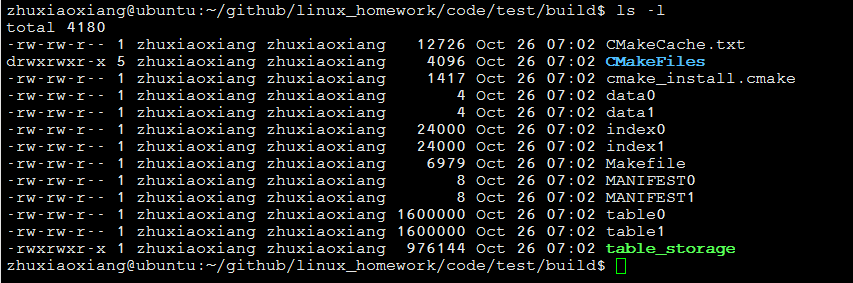
\includegraphics[height=5cm]{images/test_linux_files.png}
	\caption{输出文件(1)}
	\label{fig:test_linux_files}
\end{figure}

下面给出添加一百万条数据的测试结果,如图\ref{fig:test_linux2}所示,测试通过。生成的表数据文件、索引文件以及MANIFEST文件如图\ref{fig:test_linux_files2}所示。一百万条记录对应的表数据文件大小为1000000*800=800000000字节,索引文件大小为1000000*12=12000000。

\begin{figure}[htbp]
	\centering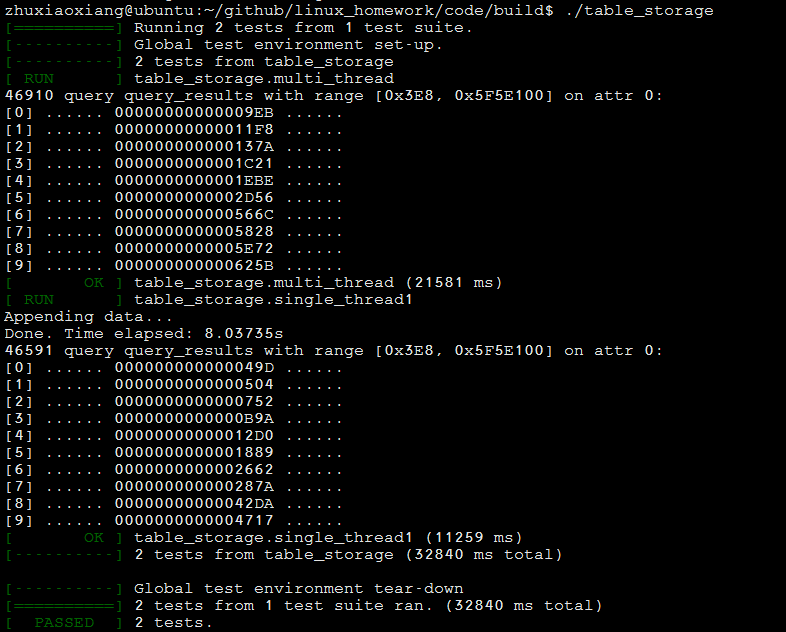
\includegraphics[height=10cm]{images/test_linux2.png}
	\caption{测试结果(2)}
	\label{fig:test_linux2}
\end{figure}

\begin{figure}[htbp]
	\centering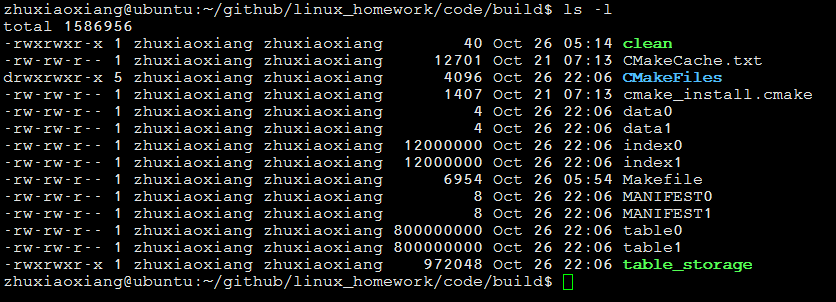
\includegraphics[height=5cm]{images/test_linux_files2.png}
	\caption{测试结果(2)}
	\label{fig:test_linux_files2}
\end{figure}

\end{document}
